\section{Conceptos previos}
En este apartado se describe la arquitectura de VMware Cloud Foundation y como estructura sus componentes\footnote{Se describen solo aquellos componentes que se utilizarán en el despliegue de Cloud Foundation.} internamente.

%%%%%%%%%%%%%%%%%%%%%%%%%%%%%%
\iffalse
En este apartado se explican aquellos conceptos de VMware Cloud Foundation necesarios para entender su funcionamiento, configuración y requisitos de la infraestructura previos al despliegue del servicio.
\fi
%%%%%%%%%%%%%%%%%%%%%%%%%%%%%%%%


%% Workload Ddomains %&%&%%%%
%%%%%%%%%%%%%%%%%%%%%%%%%%%%
\subsection{Workload Domain}
Un \textit{workload domain} consiste en una instancia lógica de un SDDC que abarca todos o parte de los recursos de uno o más clusters, cuya función es aislar el flujo de trabajo de un usuario, aplicación o un determinado tipo de tareas. Cada \textit{workload domain} se extiende sobre varios hosts y contiene su propia instancia de vCenter Server, vSAN y NSX, lo cual permite establecer políticas de control únicas para todos los \textit{workload domains} y específicas para cada uno de ellos a la vez que se simplifica la complejidad de la infraestructura. Existen \underline{tres tipos} de \textit{workload domains} que permiten aislar las tareas de gestión de la infraestructura del resto de flujos de trabajo. 

%% MANAGEMENT DOMAIN
\subsubsection{Management Domain}
\label{subsubsec:domainManagement}
Este \textit{workload domain} se crea y configura automáticamente durante el proceso de despliegue de una instancia de VMware Cloud Foundation. Su función es gestión de todos los componentes de VMware Cloud Foundation, de toda la infraestructura y del resto de \textit{workload domains} existentes en el entorno a tráves de políticas establecidas desde un único punto. Los componentes dedicados a este \textit{workload domain} son SDDC Manager, vCenter Server, dos Platform Services Controllers que son redundantes, vRealize Log Insight y un vSwitch Distributed [Fig. \ref{fig:esquemaCFComponentes}].\\
Cuando se \underline{despliega Management Domain se crean y configuran} de forma automatizada por SDDC Manager las siguientes máquinas virtuales (VM) de cada componente de Cloud Foundation:
\begin{itemize}
    \item Una VM de \textbf{SDDC Manager}: 4 vCPU, 16 GB de memoria, 800 GB de almacenamiento.
    \item Una VM de \textbf{vCenter Server}: 4 vCPU, 16 GB de memoria, 290 GB de almacenamiento.
    \item Dos instancias de \textbf{Platform Services Controller} (cada una): 2 vCPU, 4 GB de memoria, 60 GB de almacenamiento.
    \item Una VM de \textbf{NSX Manager}: 4 vCPU, 16 GB de memoria, 60 GB de almacenamiento.
    \item Tres VM de \textbf{NSX Controller} (cada una): 4 vCPU, 4 GB de memoria, 28 GB de almacenamiento.
    \item Tres VM de \textbf{vRealize Log Insight}, una en cada nodo: 8 vCPU, 16 GB de memoria, 1312 GB de almacenamiento.
\end{itemize}


%% VIRTUAL INF. DOMAIN
\begin{subsubsection}{Virtual Infrastructure Domain (VI) y Virtual Desktop Infrastructure Domain (VDI)}
\label{subsubsec:domainVI}
Este tipo de \textit{workload domain} se crea manualmente y bajo demanda desde el \textit{management domain} para dar servicio a las necesidades de cada usuario o para crear diferentes entornos con finalidades distintas. Su configuración de hardware y lógica se especifican durante su proceso de creación, permitiendo indicar la cantidad de hosts, cantidad de almacenamiento, políticas de rendimiento y disponibilidad, o configuración de la red disponibilidad, todo para satisfacer las necesidades de los usuarios que realizarán sus trabajos en él. El acceso a un \textit{VI domain} se realiza a través de vSphere Client donde su administrador puede gestionar todos los recursos asociados con ese \textit{workload domain}. Cada Virtual Infrastructure Domain cuenta con sus propios vCenter Server y un NSX Manager dedicados, que se ejecutan desde el \textit{management domain} de la infraestructura, y \textit{datastore} vSAN dedicado [Fig. \ref{fig:esquemaCFComponentes}]. La diferencia entre un \textit{virtual infrastructure domain} y \textit{virtual desktop infrastructure domain} es que el segundo incorpora el producto VMware Horizon View que, resumiendo, permite desplegar escritorios virtuales.\\
Cuando se \underline{despliega un \textit{virtual infrastructure domain} se crean y configuran} de forma automatizada por el componente SDDC Manager las siguientes máquinas virtuales (VM) de cada componente de VMware Cloud Foundation:
\begin{itemize}
    \item Una VM de \textbf{vCenter Server} en Management Domain: 8 vCPU, 24 GB de memoria, 500 GB de almacenamiento.
    \item Una VM de \textbf{NSX Manager} en Management Domain: 4 vCPU, 16 GB de memoria, 60 GB de almacenamiento.
    \item Tres VM de \textbf{NSX Controller} en el VI Domain creado (cada una):  4 vCPU, 4 GB de memoria, 28 GB de almacenamiento.
\end{itemize}

\end{subsubsection}
\begin{figure}[h!]
  \centering
  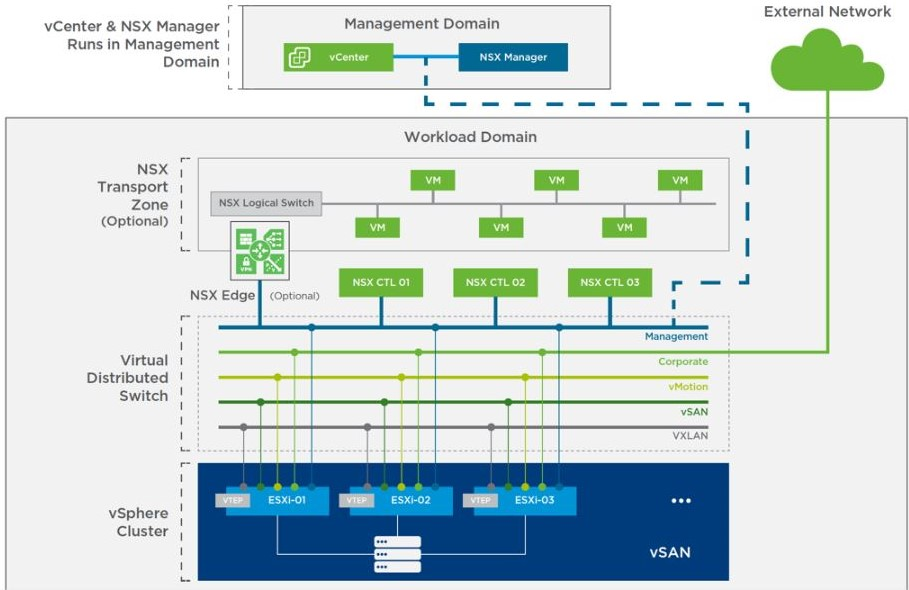
\includegraphics[width=1\textwidth]{imaxes/conceptosPrevios/WDomainStructure.JPG}
  \caption{Como se estructuran y conectan los componentes de VMware Cloud Foundation.}
  \label{fig:esquemaCFDominios}
\end{figure}
\begin{figure}[h!]
  \centering
  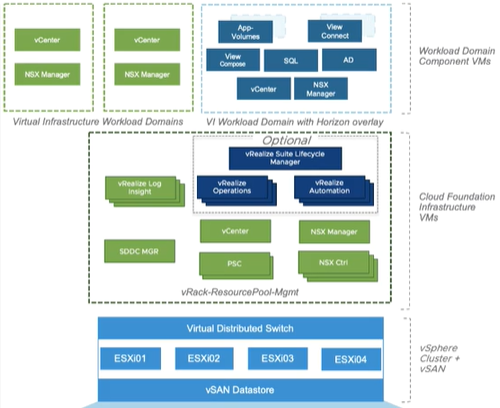
\includegraphics[width=1\textwidth]{imaxes/conceptosPrevios/workloadDomains.png}
  \caption{Componentes dedicados de cada \textit{workload domain}.}
  \label{fig:esquemaCFComponentes}
\end{figure}


\FloatBarrier

%&%%%%%%%%%%%%%%%%%%%%%%%%%%%%%%%%%%%%%%%%%%%%%%%%%%%%%%%%
%% ARQUITECTURA
\subsection{Arquitectura}
La arquitectura de VMware Cloud Foundation tiene dos posibles modelos de despliegue dependiendo del número de hosts sobre los que se despliega VMware Cloud Foundation.

%% ESTANDAR
\subsubsection{Modelo estándar}
Este modelo se utiliza cuando VMware Cloud Foundation se despliega en un entorno con siete o más hosts. Está formado por un \underline{management domain} que se despliega en uno de los hosts y que contiene todos los componentes de gestión de toda la infraestructura [Sec. \ref{subsubsec:domainManagement}], y por \underline{virtual infrastructure domains} que se crean bajo demanda sobre el resto hosts disponibles [Sec. \ref{subsubsec:domainVI}] y una vez creado se pueden ampliar o reducir sus capacidades según sea necesario. El máximo número de \underline{virtual infrastructure domains} que se pueden desplegar en una instacia de VMware Cloud Foundation es 15.

\begin{figure}[h!]
  \centering
  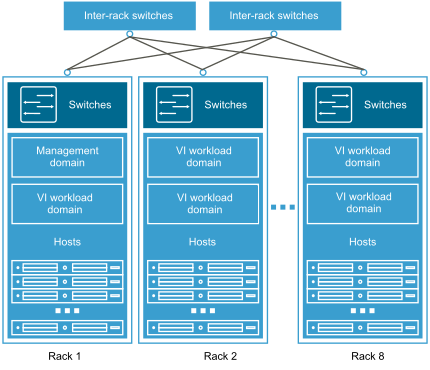
\includegraphics[width=0.75\textwidth]{imaxes/conceptosPrevios/arquitect_standarCF.png}
  \caption{Esquema del modelo de arquitectura estándar.}
  \label{fig:modelostandard}
\end{figure}

\begin{figure}[h!]
  \centering
  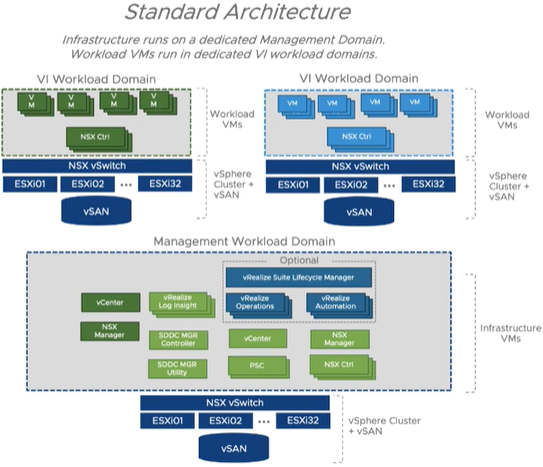
\includegraphics[width=0.85\textwidth]{imaxes/conceptosPrevios/standardArch.png}
  \caption{Estructura de los componentes en una arquitectura estándar.}
  \label{fig:standardarch}
\end{figure}
\FloatBarrier
%%%%%%%%%%%%%%%%%%%%%
%%  CONSOLIDADO
\subsubsection{Modelo consolidado}
Este modelo se despliega cuando el entorno esta formado por menos de siete nodos. En este modelo el flujo de trabajo que corresponde al \underline{virtual infrastructure domain} y al \textit{management domain} en el despliegue estándar, está colocado dentro del mismo \underline{workload domain}, es decir, solo existe un único \textit{workload domain} denominado \textit{management domain}. Este modelo se puede convertir en un modelo estándar creando un \textit{virtual infrastructure domain}. Los flujos de trabajo se mantienen aislados gracias a sus respectivos almacenes de recursos[Fig. \ref{fig:modeloconsolidated}].

\begin{figure}[h!]
  \centering
  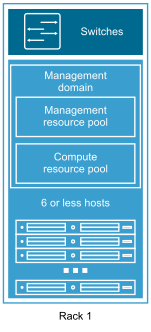
\includegraphics[width=0.25\textwidth]{imaxes/conceptosPrevios/modelConsolidated.png}
  \caption{Esquema del modelo de arquitectura consolidado.}
  \label{fig:modeloconsolidated}
\end{figure}

\begin{figure}[h!]
  \centering
  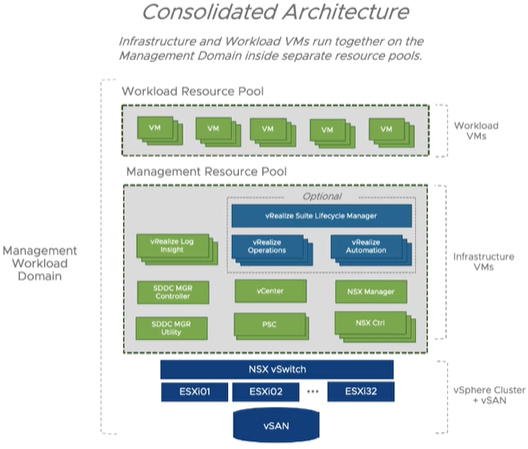
\includegraphics[width=0.85\textwidth]{imaxes/conceptosPrevios/consolidatedArch.png}
  \caption{Estructura de los componentes de una arquitectura consolidado.}
  \label{fig:consolidatedArch}
\end{figure}
\FloatBarrier


%%%% DISEÑO ARQUI. FÍSICA %%%%%
\begin{subsection}{Diseño arquitectura física}

\subsection{Tipos de clusters, zonas de disponibilidad y regiones}
Un SDDC puede estar formado por múltiples clusters que pueden ser de diferentes tipos de clusters con diferentes propósitos. Un cluster puede ocupar uno o más \textit{racks} dependiendo del nivel de escalabilidad que se requiera. Según su función, cada \textit{workload domain} se puede colocar en un cluster diferente para gestionar la alta disponibilidad y el ciclo de vida según sus necesidades. Un cluster puede ser:
\begin{itemize}
    \item \textbf{Management Cluster}: Es aquel que contiene el \textit{management domain}.
    \item \textbf{Shared Edge y Compute Cluster}: contiene el \textit{virtual infrastructure domain} con las máquinas virtuales de los usuarios y, además, incorpora los servicios de NSX necesarios para comunicarse con redes externas y con otros \textit{workload domains}.
    \item \textbf{Compute Cluster}: solo contiene el \textit{virtual infrastructure domain} con las máquinas virtuales de los usuarios.
    \item \textbf{External Storage}: se centra en proveer almacenamiento de tipo NFS, iSCSI o Fiber Channel.
\end{itemize}

Un SDDC puede estar distribuído en una o más \underline{zonas de disponibilidad}. Estas son zonas aisladas que evitan la propagación de fallos de hosts individuales a través de toda la infraestructura para establecer mayor disponibilidad. A su vez, varias \underline{zonas de disponibilidad} están agrupadas en \underline{regiones}, entornos separados por grandes distancias para tener recuperación ante desastres.\\
*******************IMAGEN AV****************\\

\subsubsection{Propiedades de la red}
El \underline{transporte de la red} de un SDDC con VMware Cloud Foundation se puede implementar en la capa dos, configurando los dispositivos físicos para funcionar directamente con los componentes de VMware, o en la capa tres del modelo OSI para usar dispositivos de transporte lógico. Cada tipo de configuración tiene sus ventajas y desventajas, pero la configuración más común en este tipo de entornos es usar el transporte de red sobre la capa 3 da más libertad a la hora de gestionar los recursos físicos de red.\\


Como VMware Cloud Foundation abstrae la red física en una red virtual, la red física debe cumplir ciertos requisitos para que la red virtualizada sea robusta. Esta se debe mantener simple con configuraciones comunes en todos los switches, uso de VLANs y uso de enrutamiento dinámico, también debe ser escalable en cuanto a cantidad de hosts, ancho de banda, o posibles rutas para alcanzar un destino. Además, se debe tener en cuenta que cada tipo de tráfico tiene características diferentes, como por ejemplo el tráfico dedicado al almacenamiento a través de IP que suele usar mayor ancho de banda, por ello es necesario distinguir cada tipo de tráfico en la capa 2 con el protocolo CoS o en la capa 3 con el protocolo DSCP. Los elementos que se deben configurar son los siguientes:
\begin{itemize}
    \item \textbf{Top of Rack Physical Switches} (TOR): se trata de un switch que está colocado dentro de un rack y a él se conectan todos los hosts que se encuentran dentro de ese rack que a su vez los conecta con el resto de la infraestructura. Estos switches se deben configurar de forma redundante para ofrecer alta disponibilidad, los puertos que se conectan a los hosts deben estar configurados como puertos troncales de forma manual, proveer servicio DHCP a cada VLAN usada por los puertos \textit{vmkernel} de \textit{management} y VXLAN, y configurar los puertos para que acepten \textit{jumbo frames}. Además, se deben configurar todas las VLANs necesarias.
    \item \textbf{Conectividad entre Regiones}: 
    \item \textbf{Conectividad entre Zonas de dispobilidad}:
\end{itemize}

\subsubsection{Características de un host ESXi}
Los hosts ESXi que se desplieguen en un cluster deben tener características físicas idénticas para hacer la infraestructura más manejable,incluyendo la configuración de almacenamiento y red.
Dos de sus interfaces de red (NIC) conla misma velocidad deben estar conectadas a la VLAN \textit{trunk}. Esto junto con el componente VMware vSphere Distributed Switch permite que el tráfico se redirija de forma óptima y que las conexiones sean redundantes. Todas las conexiones deben terner una velocidad mínima de 10 Gbit.

\end{subsection}

%%%%%DISEÑO ARQ. VIRTUAL
\begin{subsection}{Diseño arquitectura virtual}
La infraestructura virtual de un SDDC está formada por dos regiones, cada una con su propio \textit{management domain} que incluye el \textit{management cluster}, y un \textit{virtual infrastructure domain} que contiene el \textit{shared cluster} y un \textit{compute cluster}.

\subsubsection{Características de la red virtual}
La red de esta infraestructura está virtualizada por VMware NSX for vSphere que utiliza los componentes vCenter Server, NSX Manager, NSX Controllers y NSX logical switch para establecer comunicaciones y aislar el tráfico de cada flujo de trabajo. El tráfico se divide en datos de flujos de trabajo donde se segrega el tráfico que pertenece a diferentes flujos, datos de control donde se agrupa el tráfico para la configuración de dispositivos virtualizados de routing, switching y firewalls, y datos de gestión donde se incluye el tráfico dedicado a la gestión de los recuros como la gestión de máquinas virtuales.\\

Estos componentes incluyen diversos servicios que suponen una abstracción lógica de dispositivos físicos de red y que VMware Cloud Foundation utiliza para formar su infraestructura virtual. Estos servicios son los siguientes:
\begin{itemize}
    \item \textbf{Logical Switches}: permite crear segmentos abstractos que representan dominios de broadcasting donde se colocan determinadas máquinas virtuales. Su tráfico tiene asignado una única VLAN y están mapeados en todos los hosts lo cual simplifica la movilidad de las máquinas virtuales entre los hosts.
    \item \textbf{Universal Distributed Logical Router}: realiza las funciones de enrutamiento entre máquinas virtuales. Son controlados por una máquina virtual y utilizan protocolos de enrutamiento dinámico como BGP y OSPF.
    \item \textbf{Designated Instance}: host ESXi encargado de resolver las solicitudes del protocolo ARP. Es elegido por NSX Controller y se elige un host por cada VLAN existente.
    \item \textit{Edge Services Gateway}: es el encargado de proveer conectividad a través de la infraestructura física para que los componentes se puedan conectar a redes externas.
    \item \textbf{Logical Firewall}: provee mecanismos de seguridad que se asemejan a las funciones de los firewalls físicos pero con la ventaja de la virtualización, lo cual hace que su configuración sea más flexible.
    \item \textbf{Logical Load Balancer}: distribuye el tráfico entre los servidores para que el uso de recursos sea el óptimo.
\end{itemize}

\end{subsection}
\begin{subsection}{Gestión de las operaciones de la arquitectura}
En este apartado se define como se gestionan en VMware Cloud Foundation las tareas de administración de todas las partes de la infraestructura. Estas tareas se agrupan en la gestión del ciclo de vida y la recopilación de información sobre el estado de cada componente existente.

\subsubsection{Gestión del ciclo de vida}
Elementos que se encargan de administrar el ciclo de vida de los componentes:
\begin{itemize}
    \item \textbf{vSphere Update Manager}: pensado para la adminstración del entorno vSphere. Permite administrar las actualizaciones que reciben los hosts ESXi, instalar software de terceros en los hosts ESXi y actualizar el hardware virtual de las máquinas virtuales. Existe una instancia de este producto por cada vCenter Server. En su arquitectura existe otro elemento llamado \textbf{Update Manager Download Service} (UMDS) y representa un entorno con acceso a la red pública donde se descargan los archivos requeridos por vSphere Update Manager, ya que este se encuentra en un entorno aislado. Esto incrementa la seguridad y permite compartir estos archivos entre distintas instancias de vSphere Update Manager.
    
    \item \textbf{vRealize Suite Licfecycle Manager}: elemento encargado de administrar el ciclo de vida de todos los productos de vRealize de forma automatizada, esto incluye el despliegue y actualización de vRealize Operations Manager, vRealize Log Insgiht y vRealize Automation. Este se conecta a un servicio externo para descargar los archivos que se necesiten. La instancia de eeste producto reside en la la Zona de Disponibilidad 1 dentro de la Region A.
    
\end{itemize}

\subsubsection{Monitorización}
En VMware Cloud Foundation la monitorización de la infraestructura es realizada por vRealize Log Insight que provee gestión y análisis de los logs de la infraestructura. Este componente conecta con todos los prodcutos de VMware y recoge información sobre las alarmas, tareas y eventos que tienen lugar usando el protocolo syslog.\\

Su modelo de despliegue está formado por un nodo \textit{Master} y dos nodos \textit{Worker}, además, se puede habilitar alta disponibilidad su balanceador de carga \textit{Integrated Load Balancer} (ILB), este último es quien recibe las peticiones de logs de los clientes y luego las retransmite a los nodos \textit{worker} y \textit{master} para obtener la información. El producto vRealize Log Insight se despliega en la Zona de Disponibilidad 1 dentro de la Region A.





\end{subsection}


%%% CLOUD BUILDER
\subsection{Cloud Foundation Builder VM Support}
\label{subsec:cloudBuilder}
El despliegue de la plataforma VMware Cloud Foundation se realiza través de una máquina virtual llamada Cloud Foundation Builder. Esta máquina recoge la configuración que se indica en la hoja de parámetros, los valida, , despliega y configura el \underline{Management Domain}. Al final del proceso, transfiere el inventario y el control del sistema al componente SDDC Manager y esta máquina virtual puede ser eliminada.\\

\subsection{Red, almacenamiento y servicios necesarios para el despliegue}

\subsubsection{Servicios internos}
\label{subsubsec:servInterno}
Durante el despliegue Cloud Foundation, hay servicios y puertos deben estar habilitados en cada nodo ESXi para Cloud Foundation Builder (Fig. \ref{fig:puertosCB}) y SDDC Manager (Fig. \ref{fig:puertosSDDC}) puedan acceder a todos los componentes.

%%%%%%%%%%%%%%%%%%%%%%%%%%%%%%%%%%%%%%%%%%%%%%%
\iffalse
\begin{figure}[h!]
  \centering
  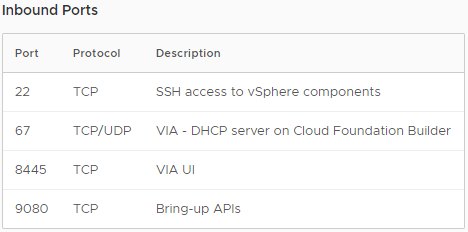
\includegraphics[width=0.7\textwidth]{imaxes/conceptosPrevios/puertosentradaCB.png}
  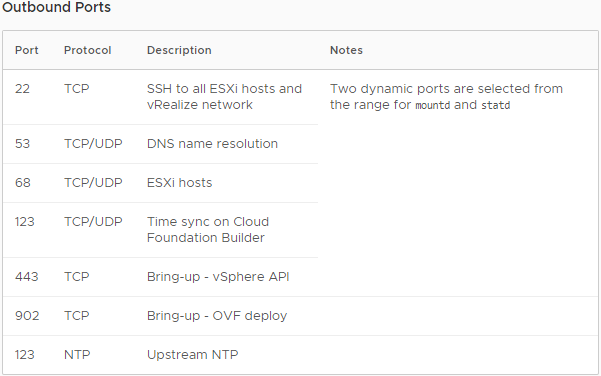
\includegraphics[width=0.7\textwidth]{imaxes/conceptosPrevios/puertossalidaCB.png}
  \caption{Servicios y puertos de entrada y salida habilitados para Cloud Foundation Builder.}
  \label{fig:puertosCB}
\end{figure}

\begin{figure}[h!]
  \centering
  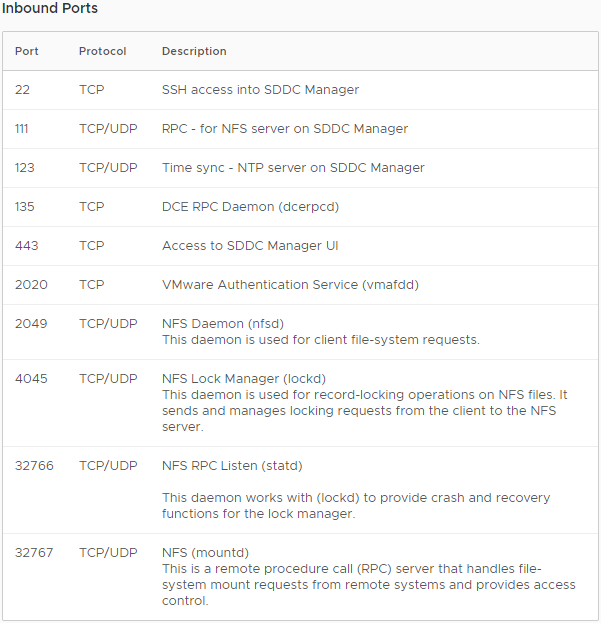
\includegraphics[width=0.7\textwidth]{imaxes/conceptosPrevios/puertosentradaSDDC.png}
  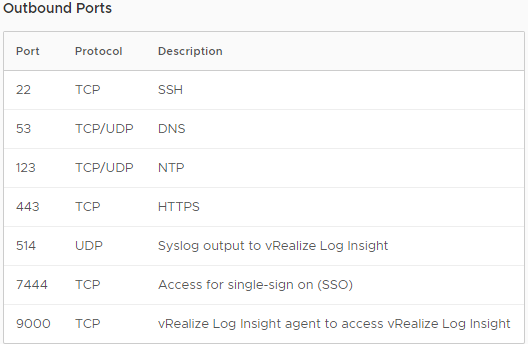
\includegraphics[width=0.7\textwidth]{imaxes/conceptosPrevios/puertossalidaSDDC.png}
  \caption{Servicios y puertos de entrada y salida habilitados para SDDC Manager.}
  \label{fig:puertosSDDC}
\end{figure}
\fi
%%%%%%%%%%%%%%%%%%%%%%%%%%%%%%%%%%%%%%%%%%%%%%%%%%%

\begin{figure}[h!]
  \centering
  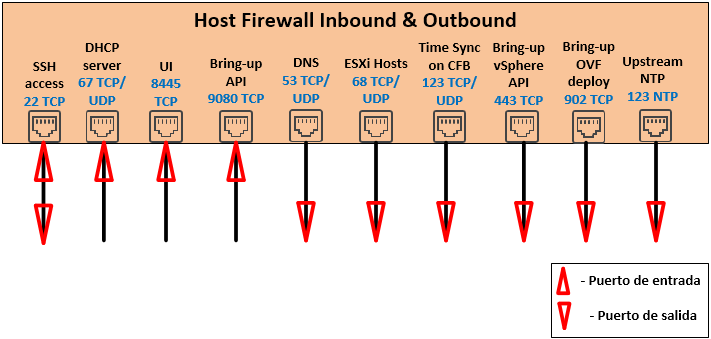
\includegraphics[width=1\textwidth]{imaxes/conceptosPrevios/firewall_CloudBuilder.png}
  \caption{Servicios y puertos de entrada y salida habilitados para Cloud Foundation Builder.}
  \label{fig:puertosCB}
\end{figure}
\begin{figure}[h!]
  \centering
  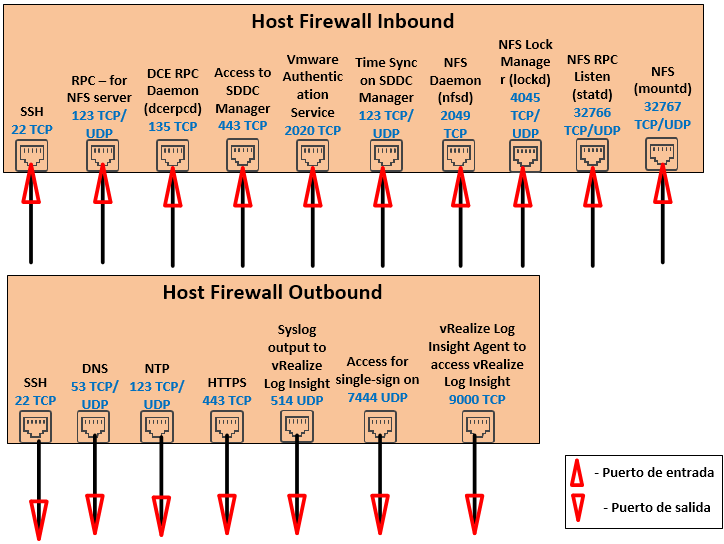
\includegraphics[width=1\textwidth]{imaxes/conceptosPrevios/firewall_SDDC.png}
  \caption{Servicios y puertos de entrada y salida habilitados para SDDC Manager.}
  \label{fig:puertosSDDC}
\end{figure}

\FloatBarrier

\subsubsection{Servicios externos}
\label{subsubsec:servExterno}
En este apartado se describen aquellos servicios necesarios para el despliegue de VMware Cloud Foundation. Estos servicios deben estar configurados antes del despliegue de VMware Cloud Foundation para que todos los componentes se puedan comunicar antes, durante y después del despliegue. Se pueden configurar en servidores instalados en máquinas virtuales dentro del entorno y estas deben tener acceso a la red \textit{VM Network}.\\
\begin{itemize}
    
    \item \textbf{Dynamic Host Configuration Protocol (DHCP)}: Permite configurar automáticamente cada puerto VMkernel de un nodo con IPv4. 
    
    \item \textbf{Domain Name Server (DNS)}: Un servidor DNS debe estar disponible para todos los componentes desde el momento de despliegue. También se debe especificar el nombre del dominio. Con esto los componentes pueden obtener tanto el nombre como la dirección IP de un elemento en la red. Los componentes y servicios de la plataforma que usan este servicio son NTP, Platform Services Controller, instancias de vCenter Server, instancias de NSX Manager y vRealize Log Insight.
    
    \item \textbf{Network Time Protocol (NTP)}: Permite la sincronizar el tiempo en todos los nodos de la infraestructura. Durante el despliegue se debe especificar la dirección IP de al menos un servidor NTP.
    
    \item \textbf{Router}: Se requiere un router con el protocolo de enrutamiento \textit{\textbf{Border Gateway Protocol}} (BGP) habilitado y configurado para compartir todas las rutas por toda la red del entorno.
    Este router debe tener configuradas cuatro interfaces para las distintas redes que se generan en la arquitectura de VMware Cloud Foundation.
    
\end{itemize}

Se puede encontrar más información sobre otros servicios opcionales en el siguiente \href{https://docs.vmware.com/en/VMware-Cloud-Foundation/3.9/com.vmware.vcf.planprep.doc_39/GUID-F022BD3C-F11C-4EE6-83EA-ABE016E7A9B9.htm}{enlace}.
\FloatBarrier

%%%%% RED 
\subsubsection{Red física}
\label{subsubsec:redFisica}
La red física debe admitir las siguientes características:
\begin{itemize}
    \item \textbf{VLAN}: etiquetado de redes VLAN (802.1Q)
    \item \textbf{Jumbo Frames}: MTU mínimo igual a 1600, aunque se recomienda que sea igual a 9000.
\end{itemize}

\subsubsection{Red lógica}
\label{subsubsec:redLogicaCF}
\iffalse
Antes del despliegue es necesario especificar varias redes que más tarde Cloud Foundation usará para automatizar la configuración de puertos \ref{Word:vmkernel} cuando se añade un nuevo host al entorno o se crea un VI Domain. Estas redes son  una dedicada al servicio \underline{vSAN}, otra dedicada a \underline{vMotion}, ota de dedicada a la gestión de los componentes y otra dedicada al tráfico de las máquinas virtuales. Los datos a especificar son la etiqueta VLAN, MTU, IP de la red, máscara, gateway y el rango de direcciones IP. Una vez creadas solo se puede modificar el rango de direcciones IP.\\
Es importante utilizar VLANs e IPs ya que es en lo que se basa Cloud Foundation para aislar cada tipo de tráfico de la infraestructura. La cantidad de subredes necesarias depende del número de Workload Domains que se creen, número de clusters y otros componentes opcionales.
\fi

Antes de iniciar el despliegue de VMware Cloud Foundation, el entorno sobre el que se instalará la plataforma debe tener configurado un vSphere Distributed Switch, una llamada \textit{Management Network} que se dedicará a la transmisión del tráfico generado entre los distintos componentes del entorno, y otra llamada \textit{VM Network} que se dedicará al tráfico generado por las máquinas virtuales que se desplieguen sobre la plataforma. La red \textit{Management Network} se puede configurar con etiquetado VLAN, en ese caso la red \textit{VM Network} debe tener la misma etiqueta VLAN. Los vSwitches creados deben tener un MTU igual a 1600 como mínimo. Además, es necesario conocer de antemano las direcciones IP que se asginarán a cada componente de la infraestructura durante el despliegue de la plataforma.


%%% ARQUITECTURA DE LA RED CLOUD FOUNDATION
\subsubsection{Arquitectura de la red}
En este apartado se describe la red que forma VMware Cloud Foundation cuando despliega las máquinas virtuales de su principales componentes y como estructura sus conexiones con los elementos ya existentes.\\
Como ya hemos visto, los diferentes servicios de esta plataforma se implementan en forma de máquinas virtuales que se conectan entre si a través de una red creada en base a los elementos de red virtualizados de VMware como \textit{Distributed Switches}, \textit{vSwitches}, \textit{vmkernels} y \textit{vmportgroups}. Esta red se denomina \textit{Management Network} y a través de esta todos 



\subsubsection{Almacenamiento}
Según la documentación de vSAN, cada host ESXi del entorno debe tener como mínimo un grupo de discos. Un nodo puede tener hasta cinco grupos de discos, dentro de los cuales debe haber al menos un disco de caché y un disco de capacidad. Cada grupo de discos puede contener hasta siete discos de capacidad.
En cuanto al tipo de disco que se debe utilizar, los discos de caché deben ser SSD y los discos de capacidad pueden ser SSD o HDD, según el modelo que se quiera implementar (All-Flash o híbrido).

%%%%%%%%%%%%%%%%%%%%%%%%%%%%%%%%%%%%%%%

